\documentclass{theme-2614084}
\usepackage{hyperref}
\usepackage{bookmark}
\usepackage{minted}

\usepackage{hyperref}

% =============================================
% Part 0 信息
% =============================================

\mathsetup{
  % 学生姓名
  student-name = {某同学},
  % 学号
  student-id = {2021xxxx},
  % 院系
  department = {电子与信息工程学院},
  % 专业
  experiment = {实验五 CMOS或非门版图设计},
  % 专业年级
  major = {集成电路设计与集成系统},
  % 日期
  % date = {\today},
}

\begin{document}

% =============================================
% Part 1  封面
% =============================================

\makecover

% =============================================
% Part 2 主文档
% =============================================

\section{实验内容与步骤}

% (注:按照内容,有截图和说明)

\subsection{实验内容}

(实验考核)

要求:

\begin{itemize}
  \item 画出或非门原理图
  \item 完成或非门的棒状图设计
  \item 完成或非门的版图设计
  \item 完成实验报告,16周交电子版
\end{itemize}

\subsection{实验步骤}

\subsubsection{准备工作}

类似实验3,此处复制了同样的文件。新建 Library,并配置 Attach 技术库。

\begin{figure}[H]
  \centering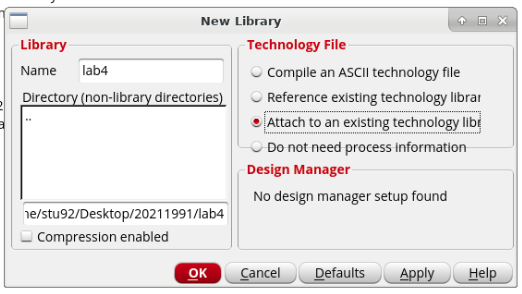
\includegraphics[width=0.6\linewidth]{1-prepare/create-new-library.png}
  \caption{Create a new library}
\end{figure}

\subsubsection{或非门原理图设计}

\begin{figure}[H]
  \centering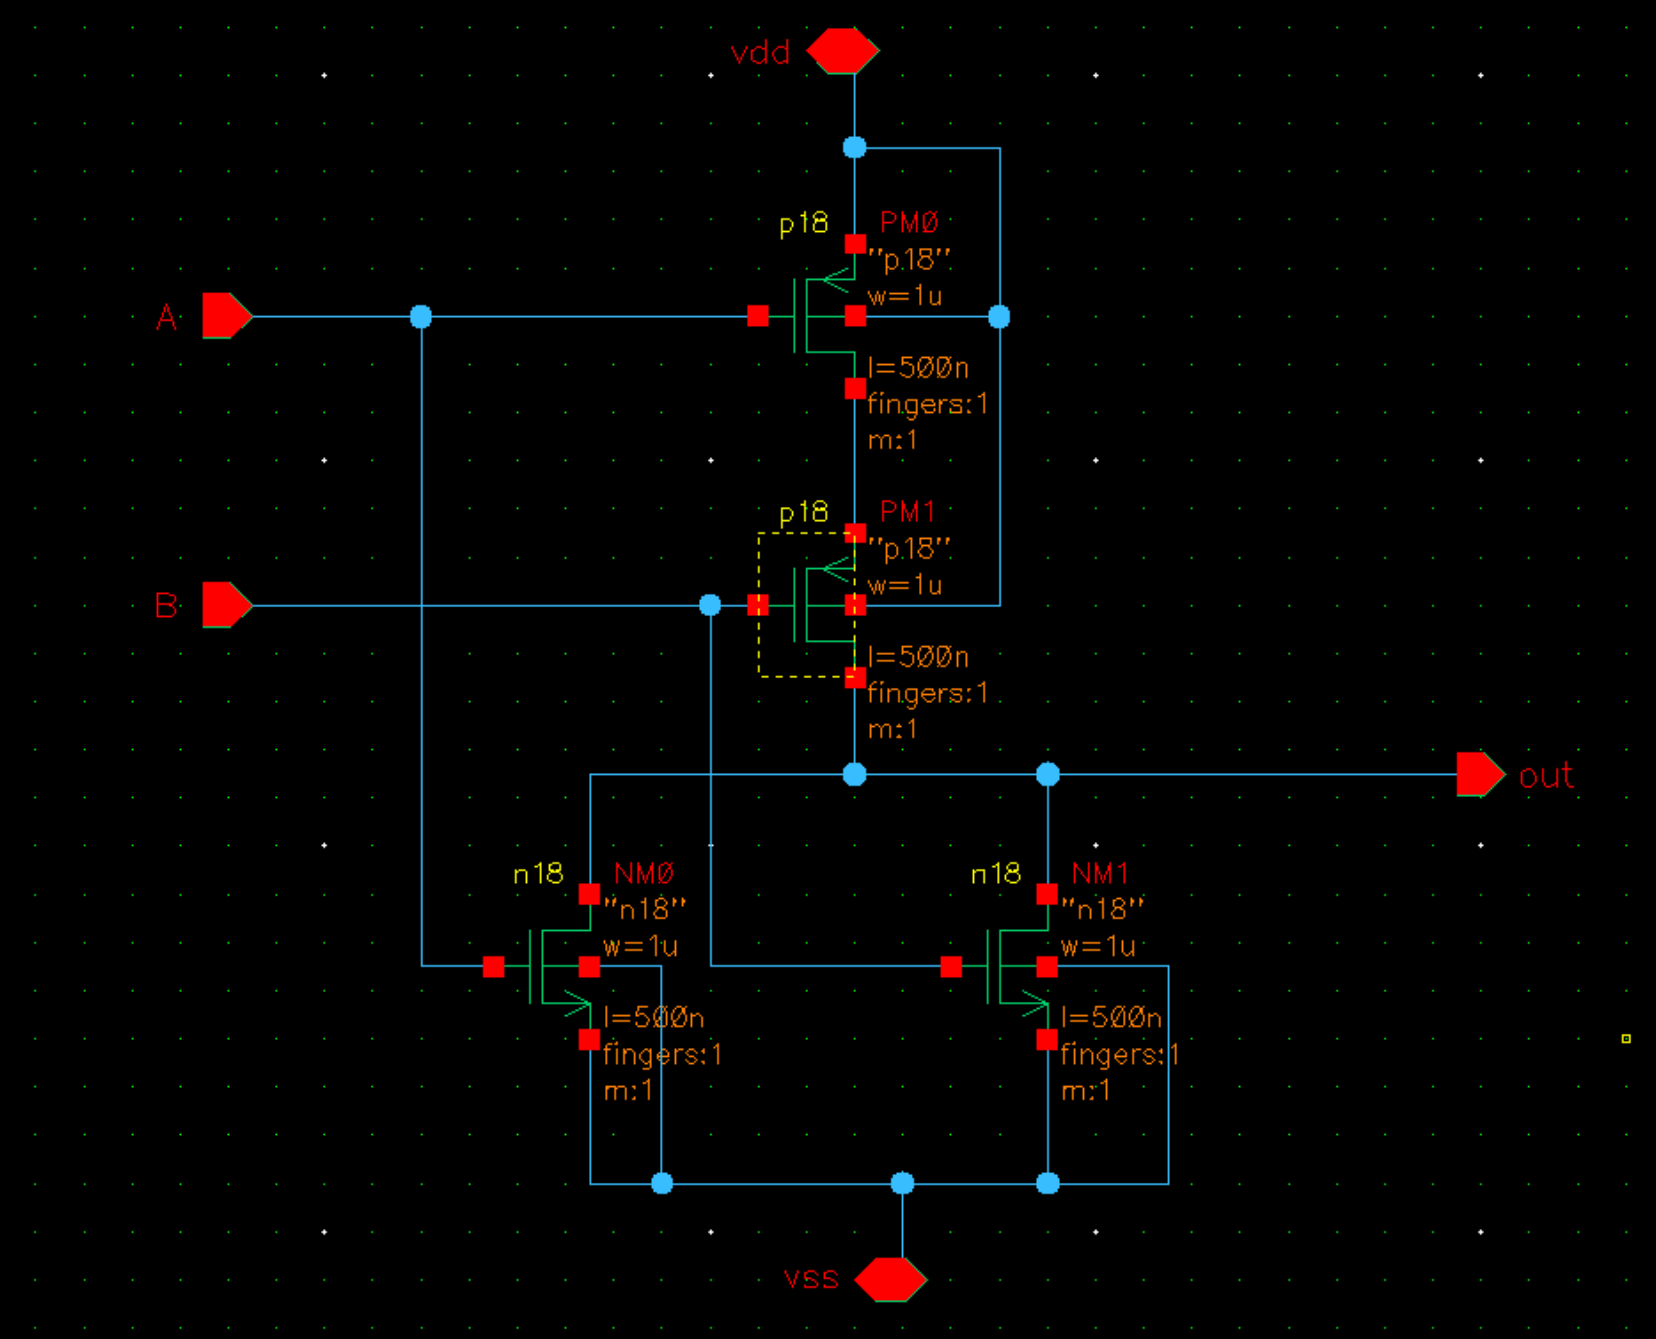
\includegraphics[width=0.6\linewidth]{2-nor-schematic/nor-schematic.png}
  \caption{NOR Schematic}
\end{figure}

\subsubsection{或非门棒状图设计}

创建或非门的 Symbol,然后画出或非门的棒状图。

下面是创建或非门的 Symbol 的步骤:

从 CellView 选择 Create Symbol 的设置

\begin{figure}[H]
  \centering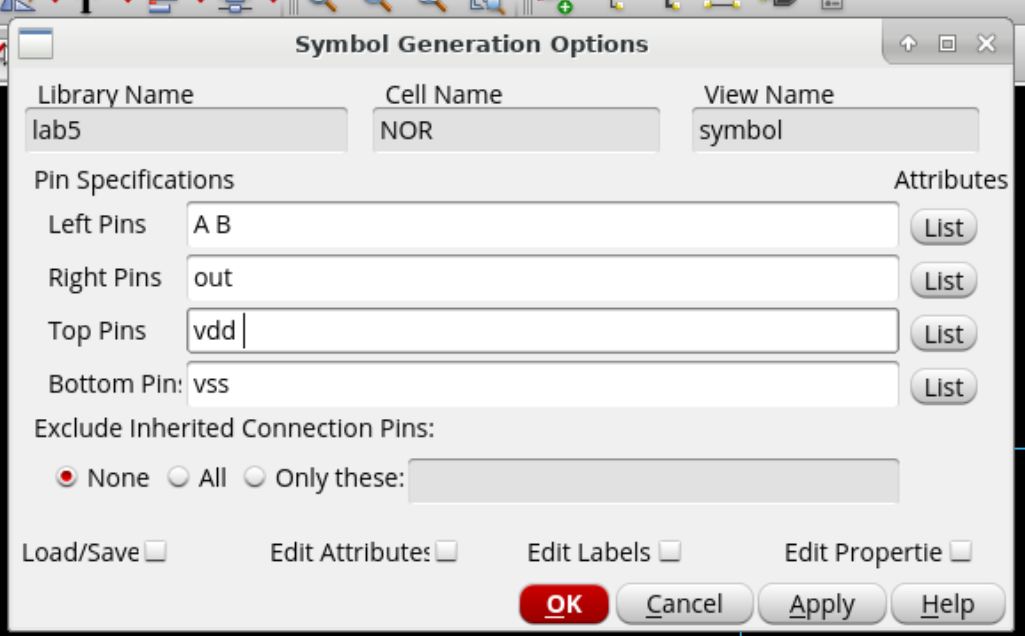
\includegraphics[width=0.6\linewidth]{3-nor-sim/nor-symbol-generation-options.png}
  \caption{NOR Symbol Generation Options}
\end{figure}

生成并编辑 Symbol

\begin{figure}[H]
  \centering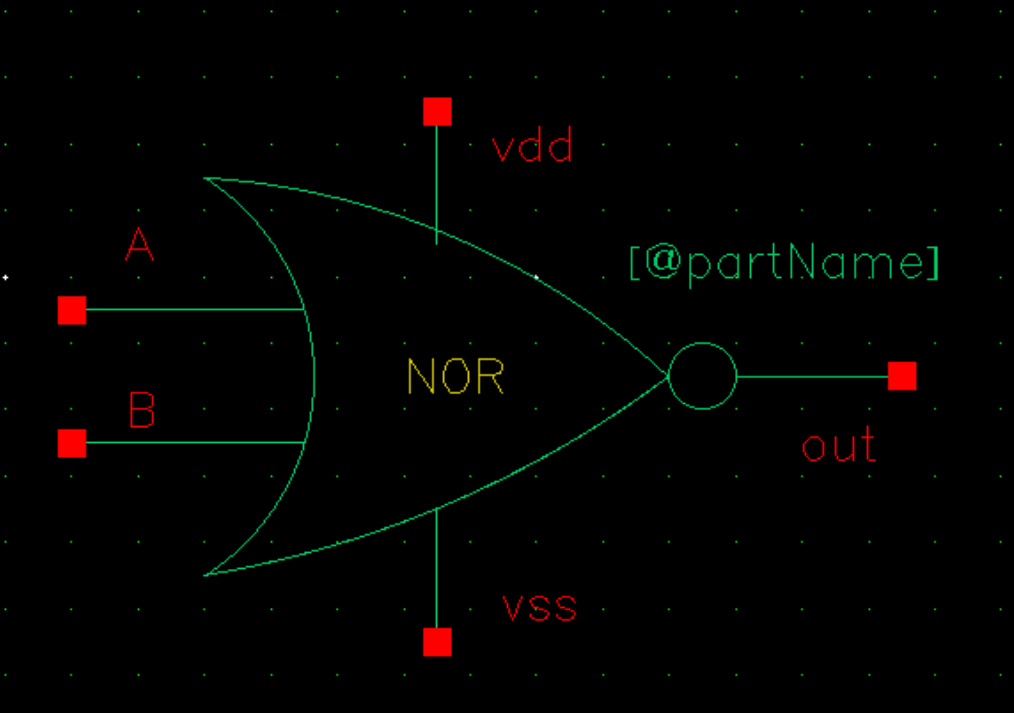
\includegraphics[width=0.6\linewidth]{3-nor-sim/nor-symbol.png}
  \caption{NOR Symbol}
\end{figure}

绘制测试用外围电路

\begin{figure}[H]
  \centering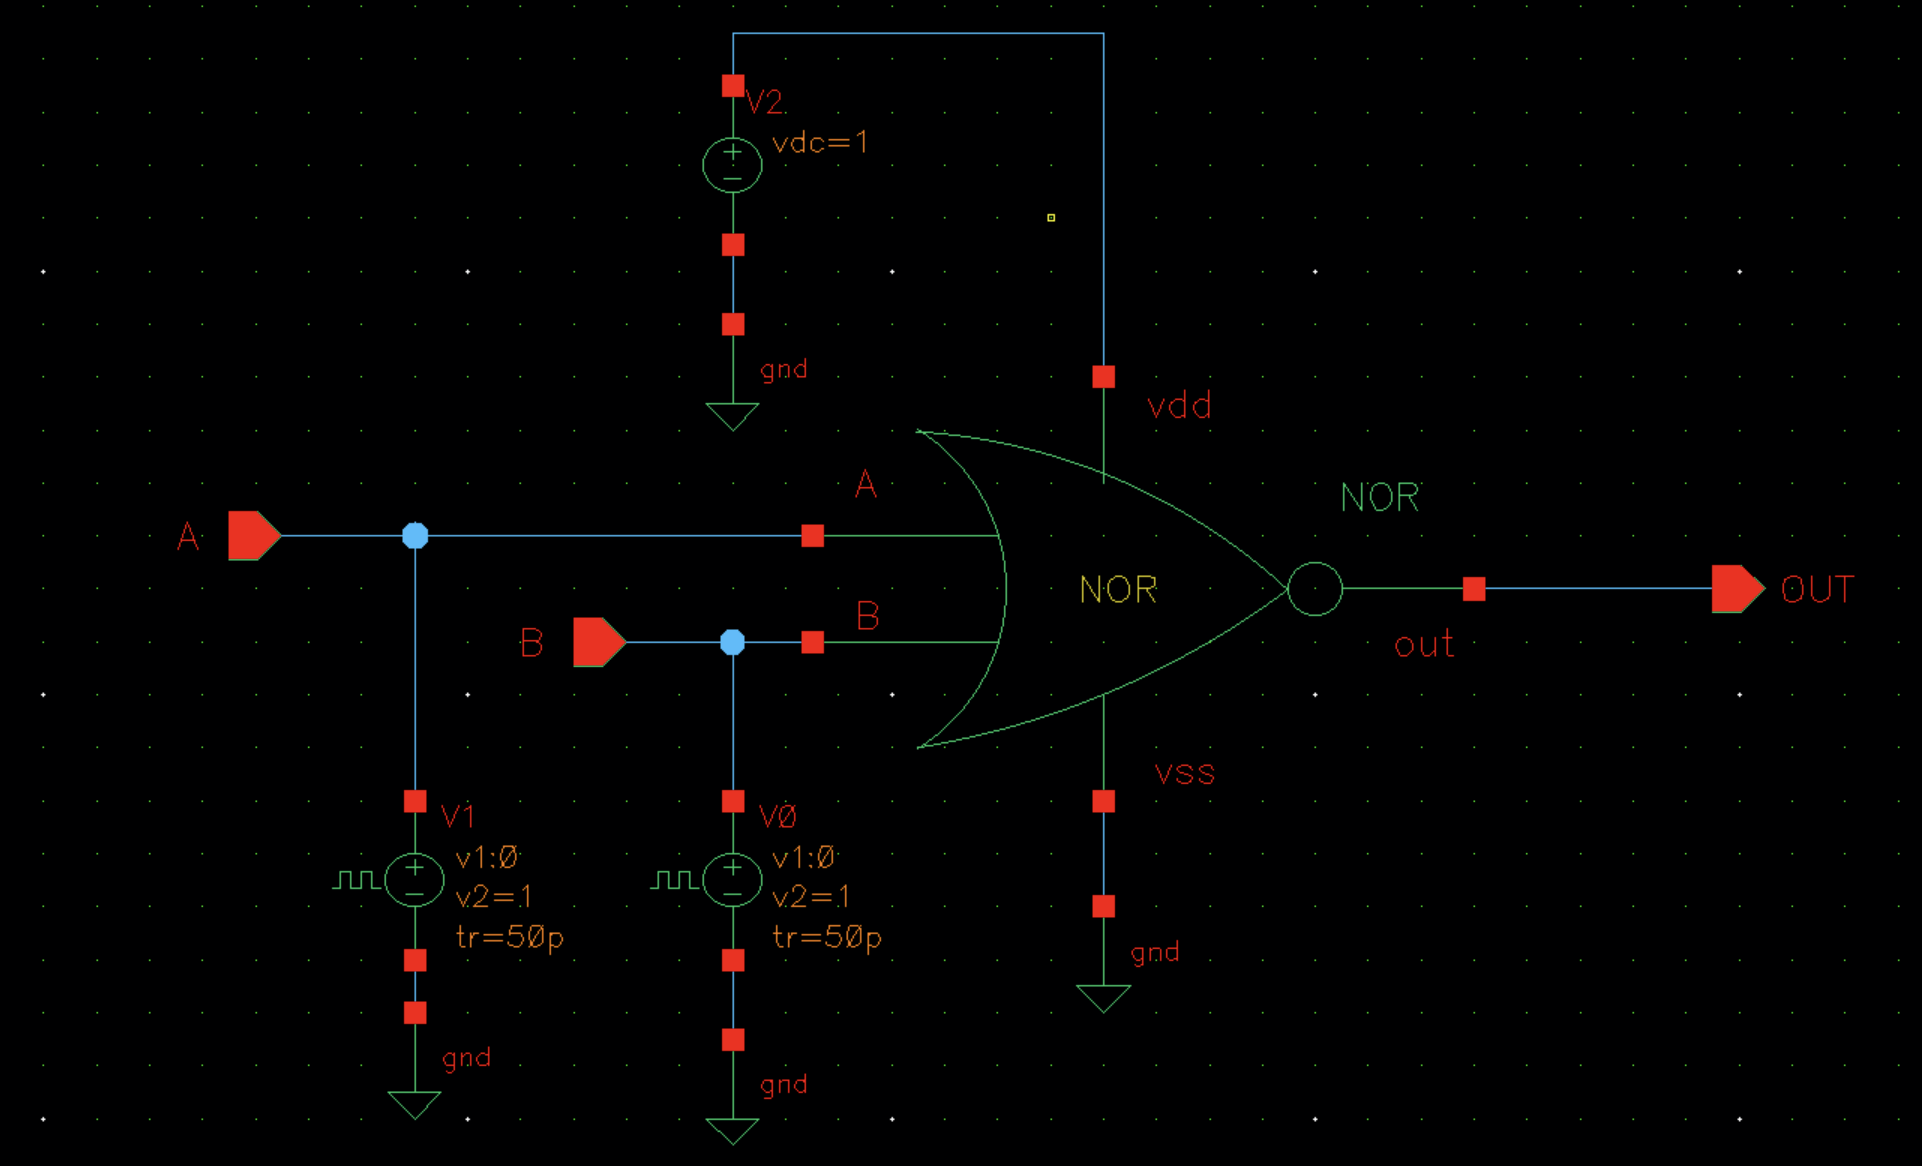
\includegraphics[width=0.6\linewidth]{3-nor-sim/nor-sim-schematic.png}
  \caption{NOR Simulation Schematic}
\end{figure}

\subsubsection{或非门版图设计}

NOR 的 Layout 设计

\begin{figure}[H]
  \centering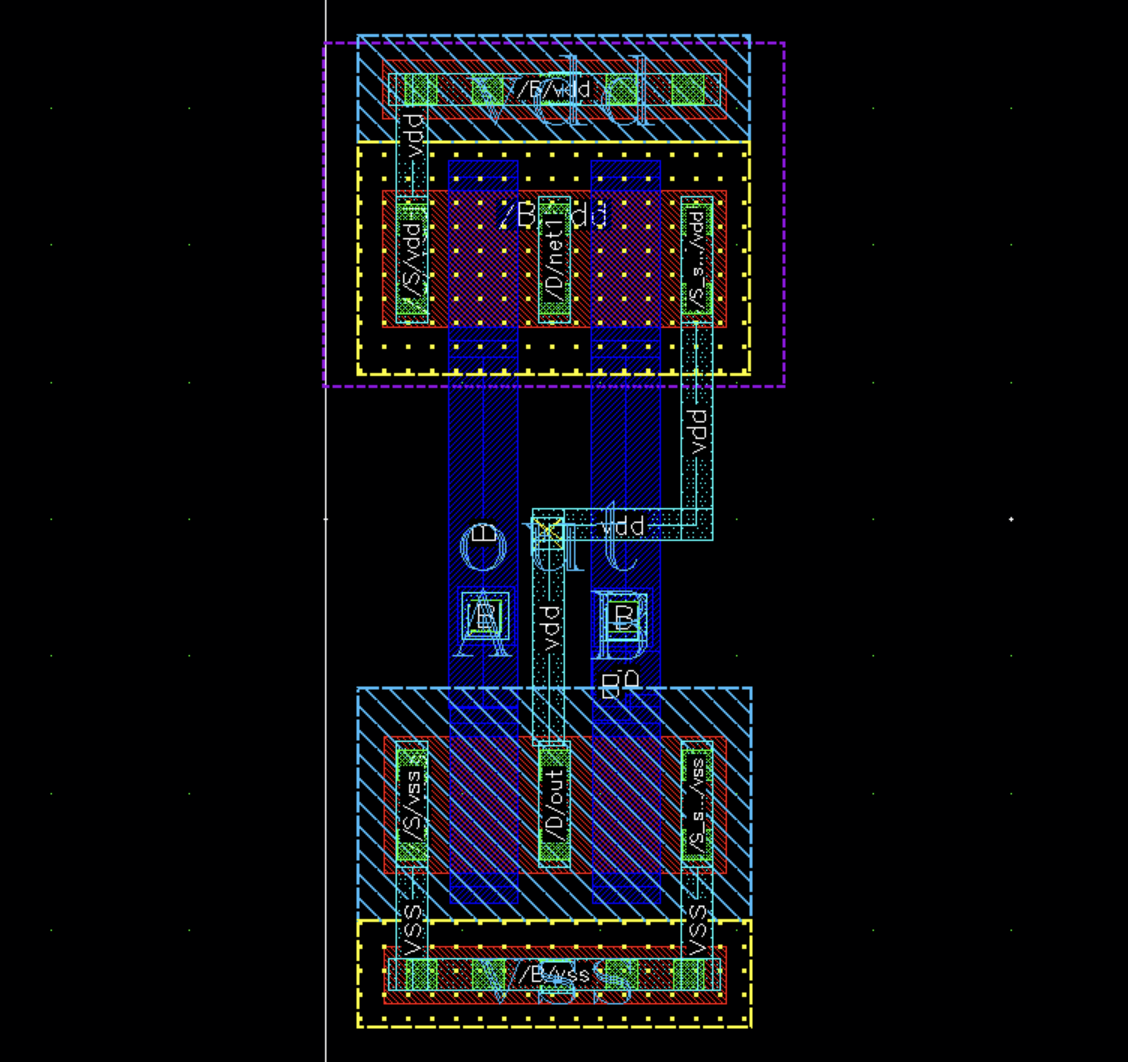
\includegraphics[width=0.6\linewidth]{4-nor-layout/nor-layout.png}
  \caption{NOR Layout}
\end{figure}

NOR 的 DRC 检查

\begin{figure}[H]
  \centering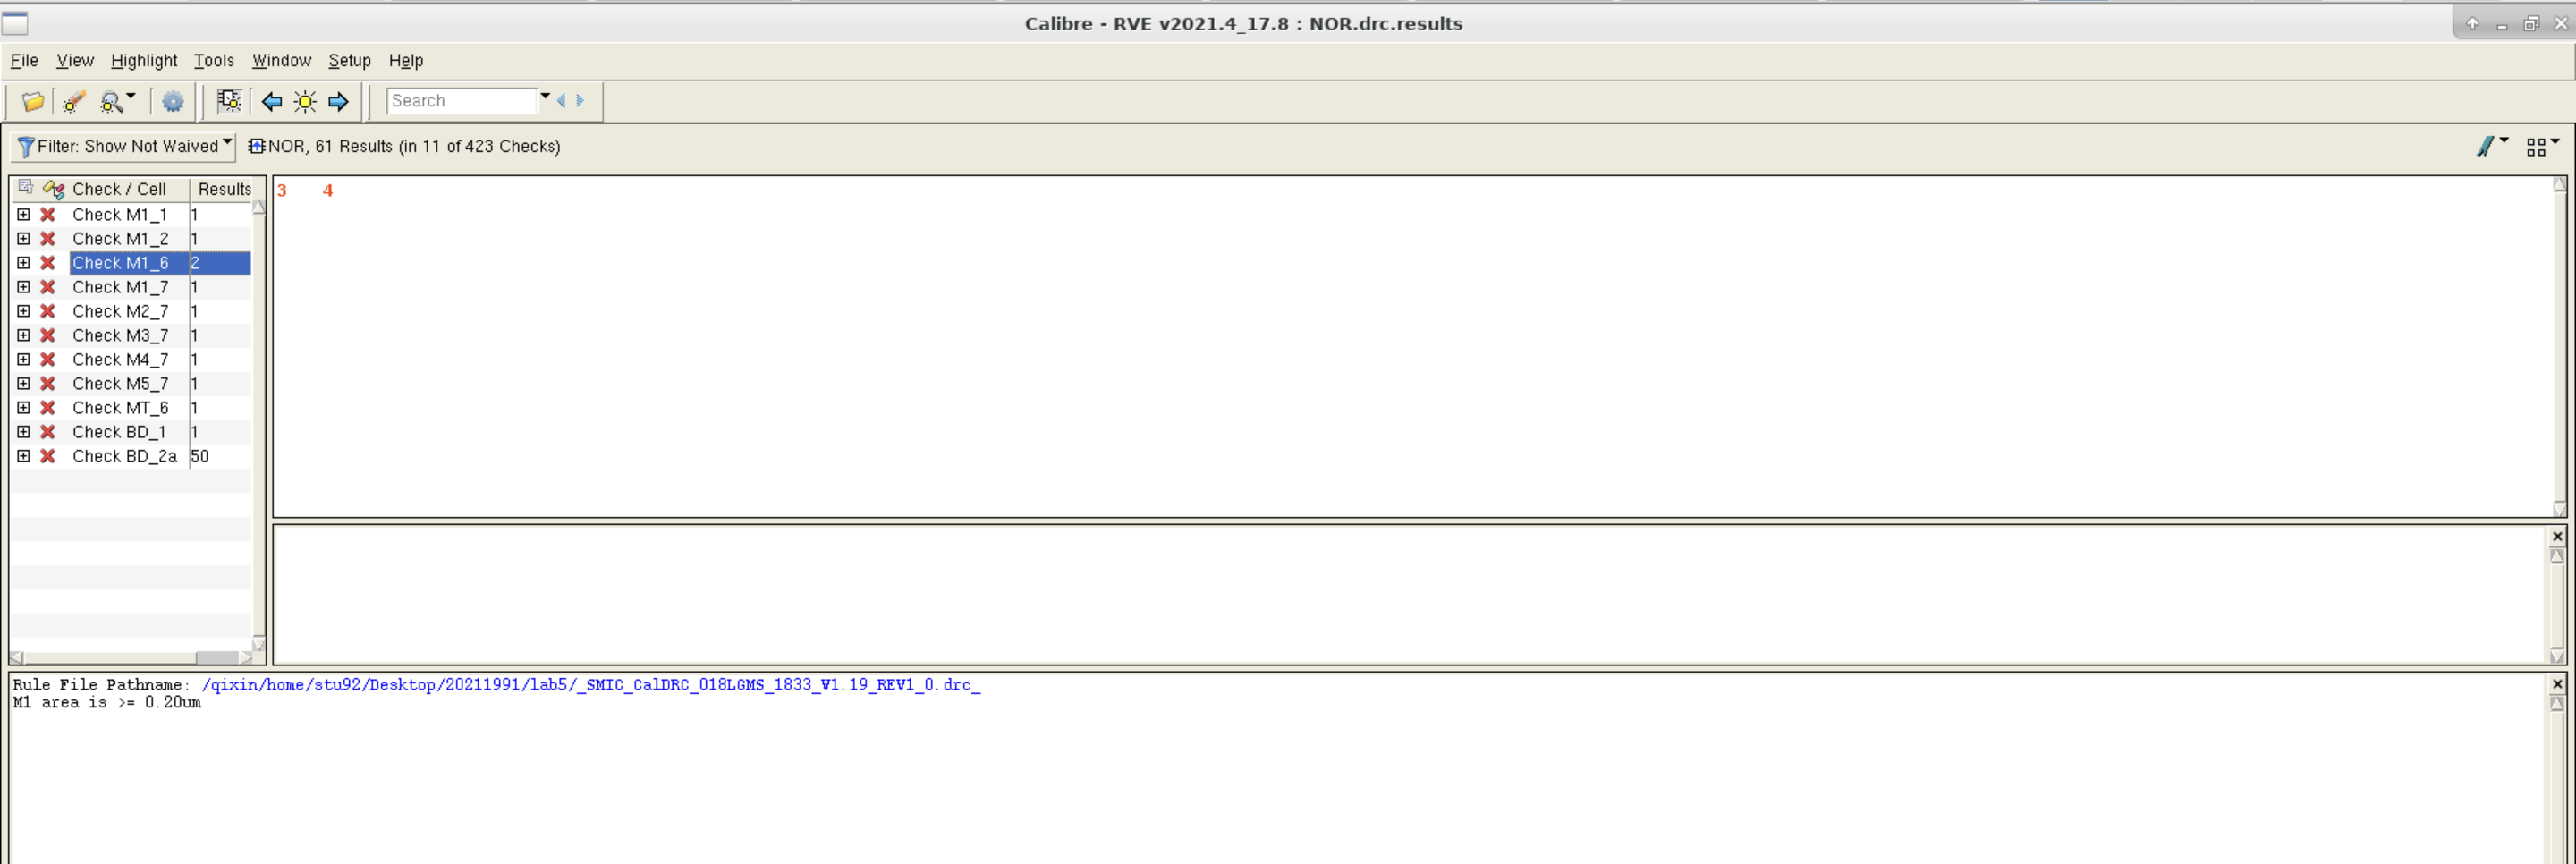
\includegraphics[width=0.6\linewidth]{4-nor-layout/nor-drc.png}
  \caption{NOR DRC}
\end{figure}

NOR 的 LVS 检查,如图中出现笑脸表示检查通过。

\begin{figure}[H]
  \centering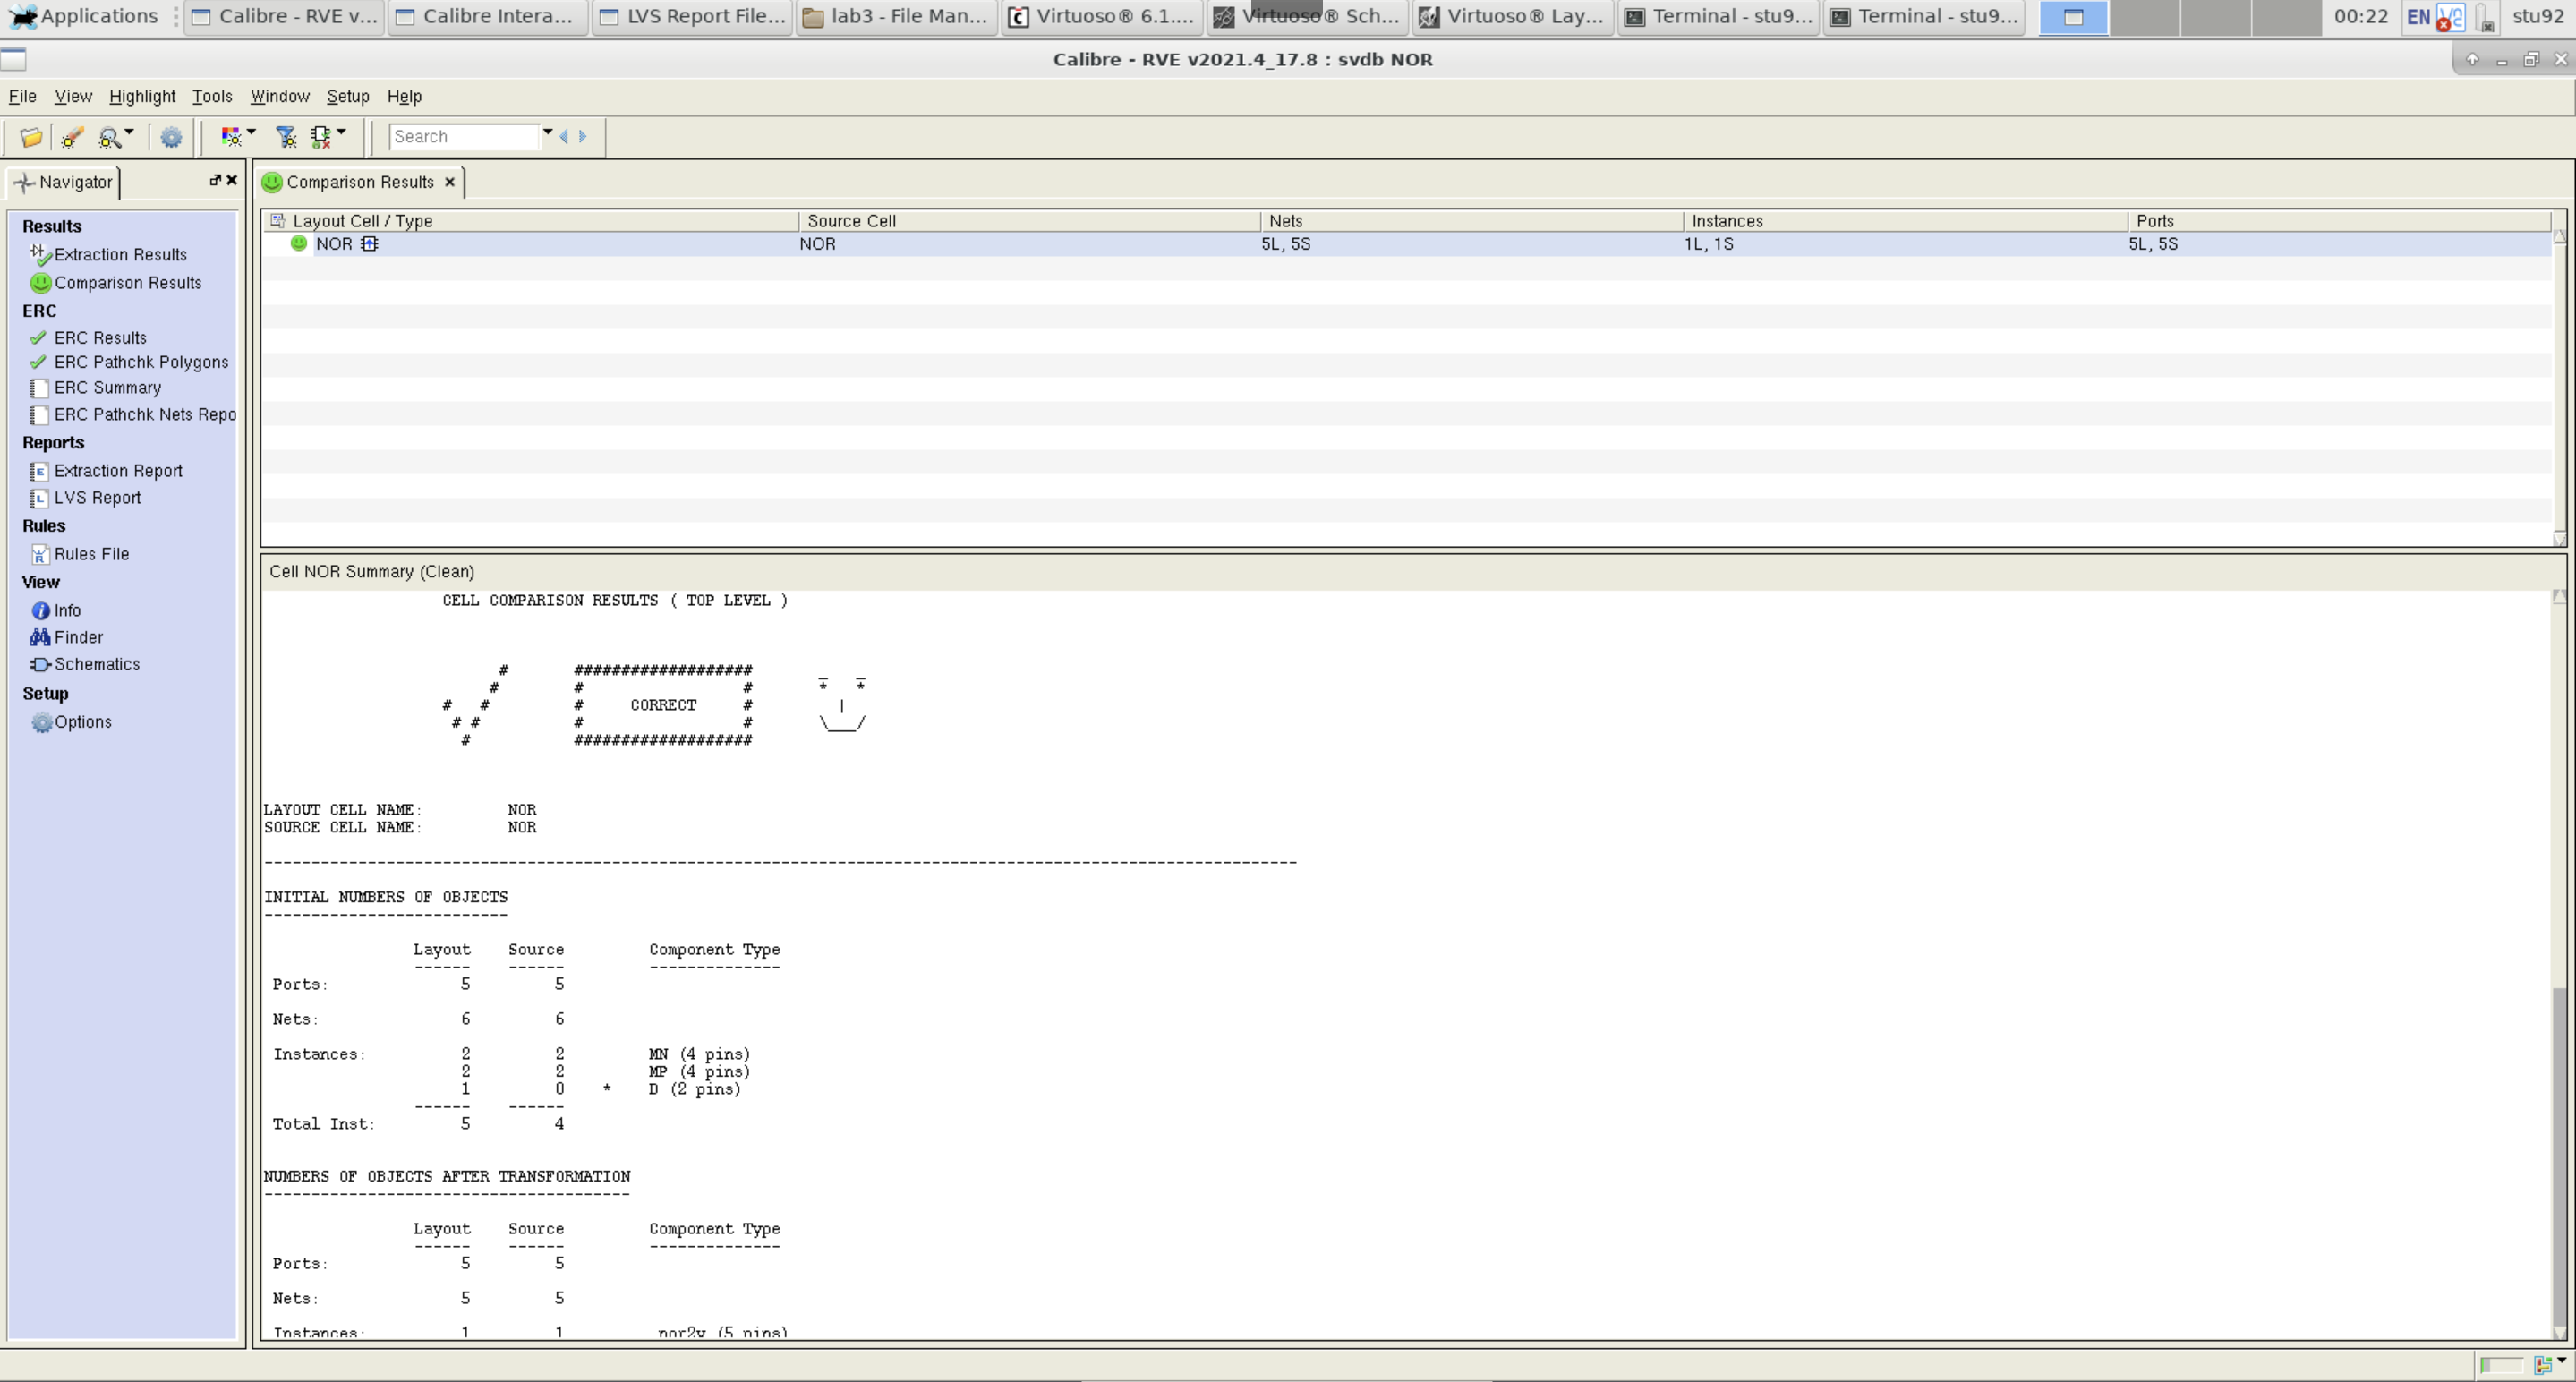
\includegraphics[width=0.6\linewidth]{4-nor-layout/nor-lvs.png}
  \caption{NOR LVS}
\end{figure}

\section{实验总结和感悟}

\subsection{遇到的问题}

The Guard Rings cannot be created because no fluid guard ring device masters exists in the technology file. Fluid guard ring device masters need to be installed as technology file devices classes before they can be instantiated in the design. Use the Install Guard Ring form to install fluid guard ring. To open the Install Guard Ring form, click Guard Ring on the Technology Tool box.

这个问题是没有读写权限导致的,实践表明,本项目不需要 Guard Ring,在当前实验环境下,也是无法被解决的。

\subsection{实验感想}

本次实验是 CMOS 或非门版图设计,通过实验,我学会了如何在 Cadence Virtuoso 中设计或非门的原理图、棒状图和版图。实验中,我遇到了 Guard Ring 的问题,但是在实验中并没有使用到 Guard Ring,所以并没有对实验造成影响。

\subsection{参考资料}

\begin{enumerate}
  \item NOR Schematic \href{https://youtu.be/px6oiPdUbMc?si=_LwnCewLOgvMCMDY}{Cadence Virtuoso: NOR Gate Schematic Design || Part-1.}
  \item NOR Layout \href{https://youtu.be/X-ke0KeekQE?si=powLM9bueuKSMTmW}{Cadence Virtuoso: Layout of NOR Gate || Part-2.}
\end{enumerate}

\href{https://www.researchgate.net/figure/The-layouts-of-2-input-standard-a-NAND-and-b-NOR-gates-where-metal-layers-are_fig1_319635790}{Figure - available from: Journal of Electronic Testing}

\end{document}
